\chapter{Weryfikacja modelowa}

Systemy tworzone przez ludzi są coraz bardziej złożone oraz odgrywają coraz większą rolę w życiu każdego z nas.
Błędy w oprogramowaniu skutkują stratami finansowymi, wizerunkowymi, opóźnieniami, a także utratą zdrowia i życia ludzi. Dowodzą temu następujące przykłady: nieudany start Ariane-5 (04.06.1996), błąd w procesorach Pentium II Intela, czy źle działająca maszyna do radioterapii spowodowała śmierć sześciu pacjentów w latach 1985-1987.


\section{Weryfikacja systemu}

Weryfikacja systemu ma na celu ustalelnie, czy projekt posiada oczekiwane właściwości. Mogą one być dość podstawowe, np. nigdy nie dojdzie do zakleszczenia lub związane z domeną, np. nie można wypłacić więcej pieniędzy niż jest na koncie. Specyfikacja dostarcza informacji jak system może oraz jak nie może się zachowywać. Oprogramowanie uważa się za poprawne, jeśli spełnia wszystkie właściwości. Schemat weryfikacji został przedstawiony na rys. \ref{fig:system_verification_scheme}.

\begin{figure}[h]
    \centering
    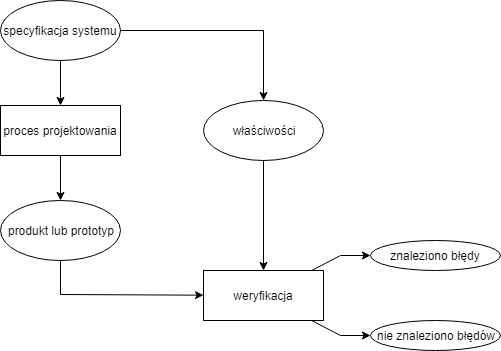
\includegraphics[height=7.5cm,keepaspectratio]{img/system_verification_schematic_view.png}
    \caption{Schemat tworzenia systemu wraz z jego weryfikacją (źródło~\cite{Bai08}).}
    \label{fig:system_verification_scheme}
\end{figure}

Podstawową formą radzenia sobie z tym problemem jest testowanie oprogramowania (testy jednostkowe, integracyjne, systemowe itp.). Polega to na uruchamianiu kodu dla różnych ścieżek wykonania, po czym waliduje się ich wyjścia z oczekiwanymi. Niestety, przetestowanie wszystkiego okazuje się praktycznie niemożliwe, zwykle sprawdzane są jedynie warunki brzegowe (stanowi to mały podzbiór wszystkich kombinacji). 


\section{Weryfikacja modelowa}

Podczas tworzenia skomplikowanych systemów, kładzie się coraz większy nacisk na testowanie poprawności oprogramowania. Metody formalne mają duży potencjał na tym polu. Ich wczesna integracja (podczas procesu projektowania) dostarcza efektywnych technik weryfikacji.
Intuicyjnie, metody formalne można rozważać jako matematykę stosowaną dla modelowania i analizy systemów informatycznych. Zapewniają one poprawność z matematyczną dokładnością.

Techniki weryfikacji bazujące na modelu opisują zachowanie systemu deterministycznie i kompletnie. Samo tworzenie pełnego modelu może wykryć luki lub niespójności.
Po jego stworzeniu, wraz z otoczającymi algorytmami, możliwe jest eksplorowanie stanów systemu.
Dzieje się to w podejściu "brute-force" - przejrzane zostają wszystkie możliwe scenariusze.
W ten sposób udowadnia się spełnialność właściwości.




\begin{figure}[h]
    \centering
    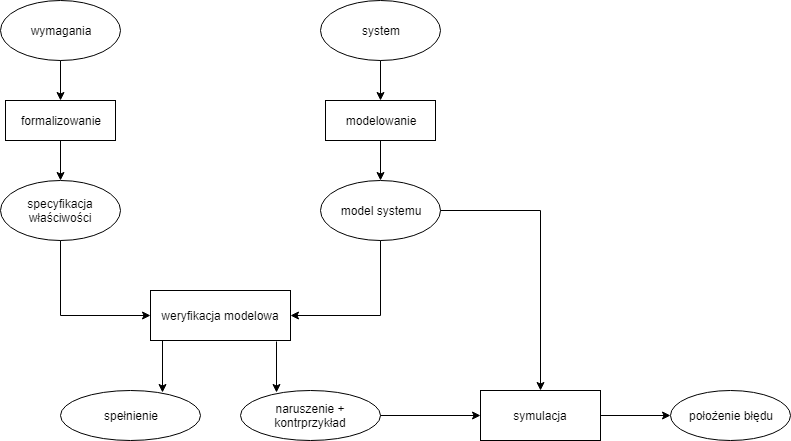
\includegraphics[height=8.8cm,keepaspectratio]{img/model_checking_approach_schematic_view.png}
    \caption{Schemat podejscia weryfikacji modelowej (źródło~\cite{Bai08}).}
    \label{fig:model_checking_scheme}
\end{figure}


\section{Logika LTL}

TODO

weryfikacja modelowa, przestrzen stanow, LTL, automaty, automaty buchiego
weryfikacja hardware i software
alogrytmy wykorzystywane w przeszukiwaniu i weryfikacji
Alvis, co to, po co

\cite{Bar12} \cite{Jac05}
przejrzec publikacje profesora




w czesci implementacji:
opis weryfikowanego systemu


A time-optimal on-the-fly parallel algorithm for model checking of weak LTL properties, in: Formal Methods and Software Engineering

 
